\section{Numerical Tests}
\label{sec:numerical}

\subsection{Problems with Known Smooth Solutions}

\subsubsection{Sine Wave: Streaming}

\subsubsection{Sine Wave: Damping}

\subsubsection{Sine Wave: Diffusion}

\subsection{Line Source}

\subsection{Homogeneous Sphere}

The homogeneous sphere test (e.g., \cite{smit_etal_1997}) considers of a sphere with radius $R$.  
Inside the sphere (radius $<R$), the absorption opacity $\sigma_{\Ab}$ and the equilibrium distribution function $f_{0}$ are set to constant values.  
The scattering opacity $\sigma_{\Scatt}$ is set to zero in this test (i.e., $\xi=1$).  
%Outside the sphere, the absorption opacity is zero.  
%The steady state solution, obtained by solving the transport equation in spherical symmetry, is given by
%\begin{equation}
%  f_{\mbox{\tiny A}}(r,\mu)=f_{0}\,\big(1-e^{-\chi_{0}\,s(r,\mu)}\big),
%  \label{distributionHomogeneousSphere}
%\end{equation}
%where
%\begin{equation}
%  s(r,\mu)
%  =\left\{
%  \begin{array}{lll}
%    r\,\mu+R\,g(r,\mu) & \mbox{if}\quad r<R, & \mu\in[-1,+1], \\
%    2\,R\,g(r,\mu) & \mbox{if}\quad r \ge R, & \mu\in[(1-(R/r)^{2})^{1/2},+1], \\
%    0 & \mbox{otherwise},
%  \end{array}
%  \right.
%\end{equation}
%and $g(r,\mu)=[1-(r/R)^{2}(1-\mu^{2})]^{1/2}$.  

\begin{figure}[h]
  \centering
%  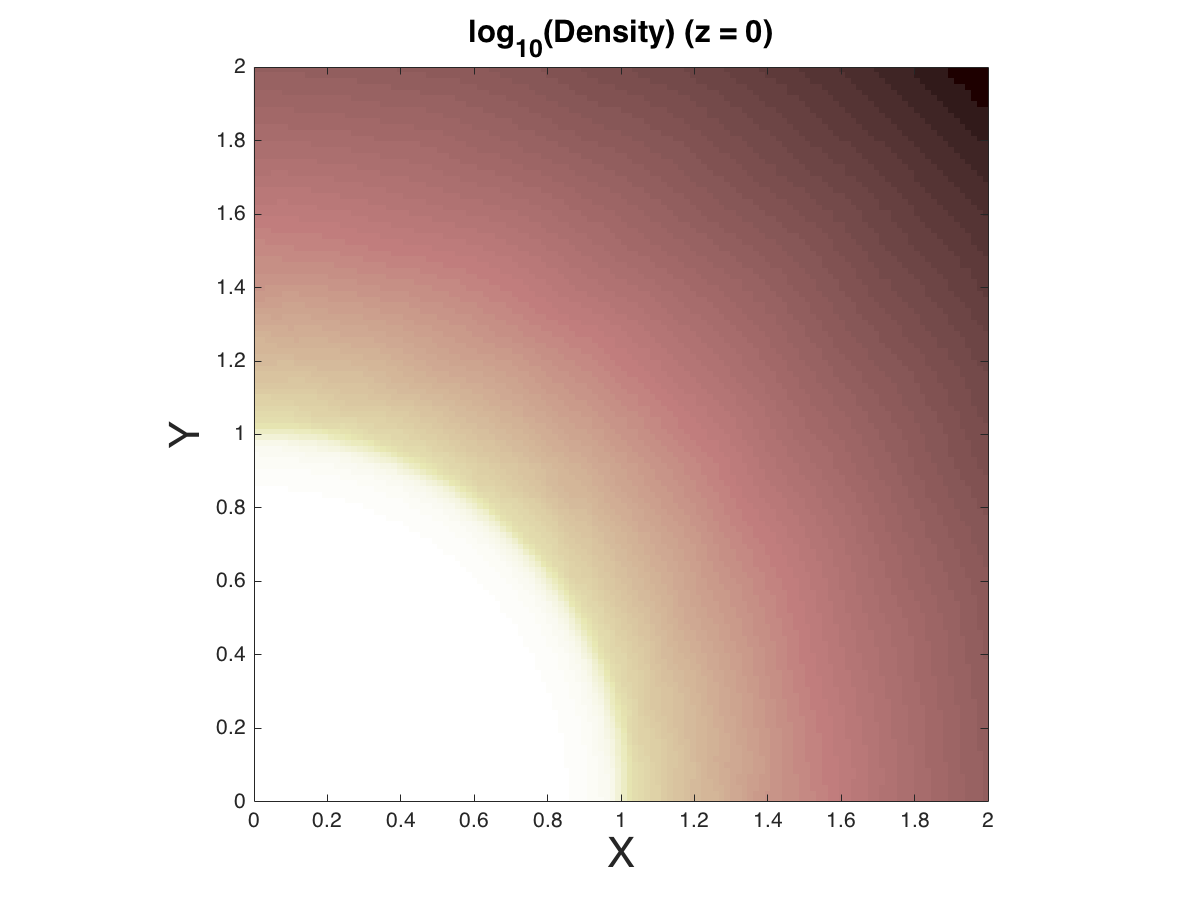
\includegraphics[width=1.0\textwidth]{figures/HomogeneousSphere_Resolution_3}
  \begin{tabular}{cc}
%    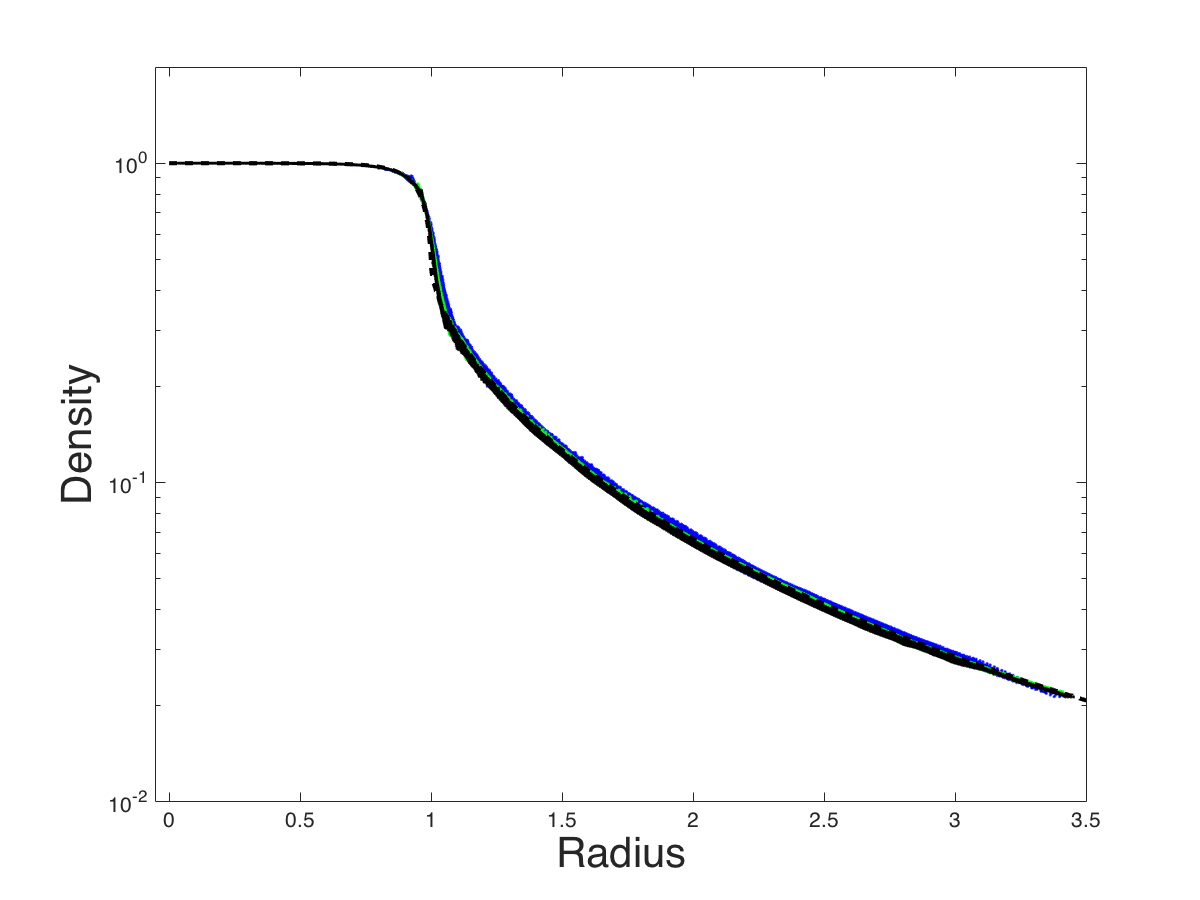
\includegraphics[width=0.5\textwidth]{figures/HomogeneousSphere_Resolution_1}
%    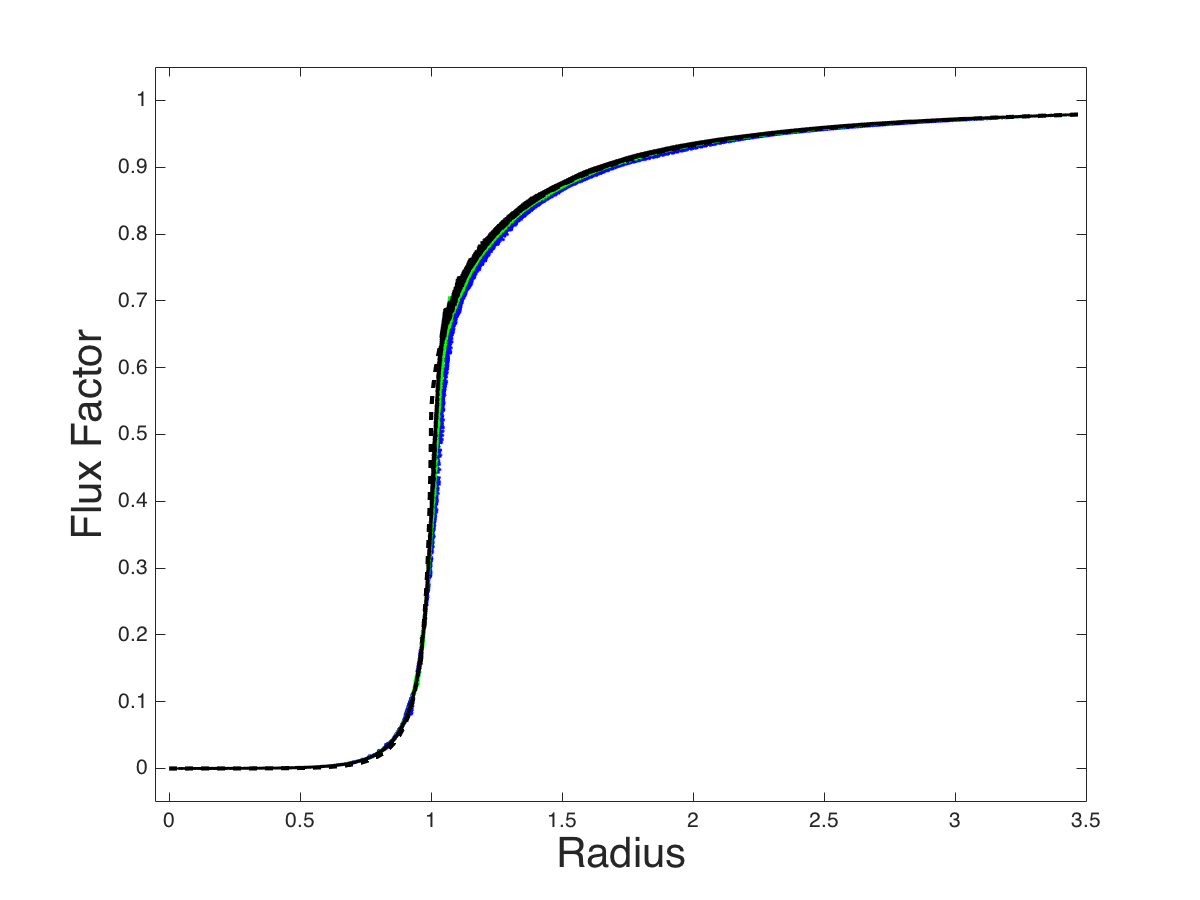
\includegraphics[width=0.5\textwidth]{figures/HomogeneousSphere_Resolution_2}
  \end{tabular}
   \caption{Homogeneous sphere problem: 32$^{3}$, 48$^{3}$, and 64$^{3}$}
  \label{fig:HomogeneousSphere_Resolution}
\end{figure}